\documentclass[
	12pt
]{article}


\usepackage{graphicx}
\usepackage{booktabs}
\usepackage{listings}
\usepackage{enumerate}
\usepackage{amsmath}
\usepackage{amsfonts}
\usepackage{amssymb}
\usepackage{enumitem}
\usepackage[utf8]{inputenc}
\usepackage[T1]{fontenc} 
\usepackage{commath}
\usepackage{xcolor}
\usepackage{float}
\usepackage{tikz-timing}
\usepackage{tikz}
\usepackage{multirow}
\usepackage{colortbl}
\usepackage{xstring}
\usepackage{listings}
\usepackage[final]{pdfpages}
\usepackage{subcaption}
\usepackage{import}
\usepackage[english]{cleveref}
\usepackage{bm}
\usepackage{wasysym}
\usepackage{stmaryrd}




\title{Modeling Population Dynamics in a Zombie Apocalypse with Dynamical Systems Theory} % Should probably change this

\date{\today}

\author{Harris Bubalo, Lea Luchterhand, Aashir Naqvi}

\begin{document}
\maketitle
\pagebreak
\tableofcontents
\pagebreak
\section{Motivation}
This report focuses on developing a simple model to to understand the population dynamics of the human race in the event of a zombie apocalypse. We model the evolution of three different sub-populations; susceptible humans, immune humans, and zombies. The focus will be on using simple assumptions to model the problem in a tractable manner, and then investigating the behavior of the system under different perturbations of the parameters of interest.
\section{Problem Definition}
We will start with a few basic assumptions. Some portion of the human population has been infected with the zombie virus, the origins of which are unknown. All humans are susceptible to being infected by the virus in the beginning. In preparation for such an event, a vaccine was developed pre-emptively and vaccination sites have been set up all over the globe. However, vaccine production and distribution is limited so only a fraction of the population can be vaccinated at any given time. Additionally, vaccinations only work pre-emptively. Once infected by the virus, a person can never be cured. Once vaccinated however, a person can not be infected again. Additionally, immune human beings give birth to susceptible human beings.

The infected population is drawn to uninfected humans and passes on the virus at a certain rate. Zombies are only interested in passing on the virus, and do not kill any humans as part of their attack. Humans on the other hand do hunt zombies and successfully eliminate them at a certain rate. 

Under these assumptions, we will now model evolutionary dynamics of each sub-population using a compartmental model approach. Going forward $H$ will represent the number of susceptible humans, $I$ will represent the number of immune humans, and $Z$ will represent the number of infected humans.

\subsection{Susceptible Humans}
% Add compartmental diagram here
The rate of change of a population is given by the by:
\begin{equation}
net \, rate = rate \, in - rate \, out
\end{equation}
The rate in is the natural birth rate of humans denoted by $a$. The rate out has a few components:
\begin{itemize}
\item The natural death rate of humans denoted as $b_H$.
\item Increased death rate as a function of population size due to competition for limited resources. We model this as a linear dependence $\gamma(H+I)$
\item The vaccination rate of susceptible humans $c_I$.
\item The infection rate of susceptible humans. This is a function of the number of infected humans in the system $c_zZ$
\end{itemize}
The rate equation becomes:
\begin{equation}
\frac{dH}{dt} = a(H+I)-b_HH-c_IH-\gamma H(H+I)-c_ZHZ
\end{equation}
If we let the $r = a-b_H$, the above can be simplified as:

\subsection{Immune Humans}
For immune humans we assume the same natural death rate as susceptible humans. There is also an influx of immune human beings from vaccinations. The population equation becomes:

\begin{equation}
\frac{dI}{dt} = c_IH-b_HI-\gamma I(H+I)
\end{equation}

\subsection{Infected Humans}
For infected humans, the birth rate is the infection rate of new humans $c_ZH$. The death rate is the rate at which they are hunted by humans which is a function of the human population. Denote this as $b_z(H+I)$. The population dynamics are then given by:

\begin{equation}
\frac{dZ}{dt} = (c_ZH-b_Z(H+I))Z
\end{equation}

\section{Analysis}
	\subsection{Analyzing the system analytically}
		\subsubsection{Validity of the model}
			A useful way to analyze this system is to look at the values of any two variables holding the third constant or zero.
			Let $H= 0$, then:
			\begin{align*}
				\frac{dH}{dt} &=aI\\
				\frac{dI}{dt} &= I(-b_H-\gamma I)\\
				\frac{dZ}{dt} &= -b_z IZ
			\end{align*}
			In this case, no new immune or infected humans are produced. However, the population of susceptible humans is increasing as the existing immune humans reproduce. \\
			For $I=0$:
			\begin{align*}
				\frac{dH}{dt} &= H(a-b_H-c_I-\gamma H)-c_z HZ\\
				\frac{dI}{dt} &= c_IH\\
				\frac{dZ}{dt} &= Z(c_ZH-b_ZH)
			\end{align*}	
			This simply says that the system remains the same, except that immune humans do not compete for resources with uninfected humans and they do not hunt zombies.\\
			For $Z=0$:
			\begin{align*}
				\frac{dH}{dt} &= a(H+I)-b_HH-c_IH-\gamma H(H+I)\\
				\frac{dI}{dt} &= c_IH+(-b_H-\gamma(H+I))I \\
				\frac{dZ}{dt} &= 0
			\end{align*}
			This is simply two competing logistic growth models. All three situations appear to be plausible.
		\subsubsection{Finding the equilibrium solutions}
We can find the equilibrium solutions to this system by looking at the nullclines and where they intersect. The nullcline from setting $\frac{dH}{dt}=0$ is given by the equation:
\begin{equation}
a(H+I)-b_HH-c_IH-\gamma H(H+I)-c_ZHZ=0
\end{equation}
For $\frac{dI}{dt}=0$, we have the quadratic form:

\begin{equation}
c_IH+(-b_Z-\gamma(H+I))I = 0
\end{equation}
Setting $\frac{dZ}{dt}=0$ gives us:
\begin{equation}
Z=0, I = H \left(\frac{c_z-b_z}{b_z}\right)
\end{equation}
The easiest way to evaluate the equlibrium points is to start with the nullclines from $\frac{dZ}{dt}=0$. The first solution $Z=0$ is not interesting from the perspective of this model since a world without zombies would not require a vaccination rate, nor a distinction between immune and susceptible humans. Hence, we will analyze  the case when $I = H \left(\frac{c_z-b_z}{b_z}\right)$. For simplicity, we will let $d_z = \left(\frac{c_z-b_z}{b_z}\right)$ so $I=d_ZH$. Substitute this into the equation $\frac{dI}{dt}=0$:
			\begin{align*}
				\frac{dI}{dt}= 0 &=  c_IH-b_HI-\gamma I(H+I) \\
				\Leftrightarrow 0&= c_IH-b_Hd_ZH,-\gamma d_ZH(H+d_ZH)\\
			\end{align*}
This gives us:
			\begin{align*}
				\Leftrightarrow H=\frac{c_I-b_Hd_z}{\gamma d_Z(1+d_Z)}\\
				\Rightarrow I =  \frac{c_I-b_Hd_z}{\gamma (1+d_Z)} 
			\end{align*}
Finally, substitute both values into the nullcline equation from $\frac{dH}{dt}$ to get $Z$. To simplify, we will start by first substituting $I=d_ZH$:
			\begin{align*}
				\frac{dH}{dt} = 0 &= a(H+I)-b_HH-c_IH-\gamma H(H+I)-c_ZHZ=0\\
				\Leftrightarrow 0&= aH(1+d_Z)-b_HH-c_IH-\gamma H^2(1+d_Z)-c_ZHZ
			\end{align*}
One of the solutions here is $H=0$, which leads to the trivial equilibrium point $(0,0,0)$. The other solution is given by solving the equation:

\begin{align*}
a(1+d_Z)-b_H-c_I-\gamma H(1+d_Z)-c_ZZ = 0\\
\Leftrightarrow c_ZZ = a(1+d_Z)-b_H-c_I-\gamma H(1+d_Z)
\end{align*}
Substitute in $H=\frac{c_I-b_Hd_z}{\gamma d_Z(1+d_Z)}$:
\begin{align*}
c_ZZ&=a(1+d_Z)-b_H-c_I-\frac{c_I-b_Hd_Z}{d_Z}\\
\Leftrightarrow Z&=\frac{(ad_Z-c_I)(1+d_Z)}{c_Zd_Z}
\end{align*}
The equilibrium solutions $(H,I,Z)$ are $(0,0,0)$ and $(\frac{c_I-b_Hd_z}{\gamma d_Z(1+d_Z)},  \frac{c_I-b_Hd_z}{\gamma (1+d_Z))} , \frac{(ad_Z-c_I)(1+d_Z)}{c_Zd_Z})$ where $d_z = \left(\frac{c_z-b_z}{b_z}\right)$.
\subsubsection{Stability Analysis}

We can get a sense for the local stability of each equilibrium point by linearizing the system around that point. The system:
\begin{equation}
\frac{dH}{dt} = a(H+I)-b_HH-c_IH-\gamma H(H+I)-c_ZHZ
\end{equation}

\begin{equation}
\frac{dI}{dt} = c_IH-b_HI-\gamma I(H+I)
\end{equation}
\begin{equation}
\frac{dZ}{dt} = (c_ZH-b_Z(H+I))Z
\end{equation}
Has the Jacobian:
\begin{equation}
J = \begin{bmatrix}
r-2H\gamma - Zc_Z - c_I - \gamma I & r-H\gamma & -Hc_Z \\
-I\gamma + c_I & -2I\gamma - b_H - \gamma H & 0 \\
 Z(-b_Z + c_Z) & -Zb_Z & Hc_Z - b_Z(H + I)
\end{bmatrix}.
\end{equation}

For our first equilibrium solution $(0, 0, 0)$, the Jacobian is:

\begin{equation}
J=\begin{bmatrix} r-c_I& 0 & 0 \\ c_I & - b_H & 0 \\ 0 & 0 & 0 \end{bmatrix}
\end{equation}
Since this is an lower triangular matrix, the eigenvalues are the diagonal elements of the matrix. So $\lambda_1=r-c_I$. $\lambda_2=-b_H$, $\lambda_3=0$. In order for the solution to be stable, all eigenvalues must have negative real parts. In this case, one eigenvalues is always $0$, which makes the linearized analysis indeterminate. However, we can deduce from knowledge of the system that if all populations are $0$, then there will be no changes in the population for small perturbations from that point. Hence, the point is locally stable.

Due to the complexity of the Jacobian and the second equilibrium solution, $(\frac{c_I-b_Hd_z}{\gamma d_Z(1+d_Z)},  \frac{c_I-b_Hd_z}{\gamma (1+d_Z))} , \frac{(ad_Z-c_I)(1+d_Z)}{c_Zd_Z})$ where $d_z = \left(\frac{c_z-b_z}{b_z}\right)$, we choose to instead examine the Jacobian under reasonable parameter values. Our chosen values are:

\begin{equation}
(a,b_h,\gamma,c_i,c_z,b_z)=(1.5,0.2,0.01,0.5,0.02,0.01)
\end{equation}

Evaluating $H$, $I$, and $Z$ for the equilibrium solution with these parameter values, we get:

\begin{equation}
    H = \frac{0.5-0.2\cdot1}{0.01\cdot1\cdot(1+1)} = 15
\end{equation}
\begin{equation}
    I = \frac{0.5-0.2\cdot1}{0.01\cdot(1+1)} = 15
\end{equation}
\begin{equation}
    Z = \frac{(1.5\cdot1-0.5)(1+1)}{0.02\cdot1} = 100
\end{equation}

Substituting the parameter values and the values of $H$, $I$, and $Z$ into the Jacobian, we have:

$$
J=\begin{bmatrix} 1.5-0.2-0.5-0.3-0.15-2 & 1.5-0.2-0.15 & -0.3 \\ 0.5 - 0.15 & -0.2-0.3-0.15 & 0 \\ 2-1 & 1 & 0.3-0.15-0.15 \end{bmatrix}
$$

$$
J=\begin{bmatrix} -1.65 & 1.15 & -0.3 \\ 0.35 & -0.65 & 0 \\ 1 & 1 & 0 \end{bmatrix}
$$

The eigenvalues are approximately $\lambda_1=-1.8664$, $\lambda_2=-0.2168+0.3372i$, and $\lambda_3=-0.2168-0.3372i$. Because the real component of each of these eigenvalues is negative, the equilibrium solution is \textbf{stable} for the given parameter values.

\section{Numerical Analysis}
The stability of this equilibrium solution can also be seen in a numerical approximation. Let's assume a population of 100 regular humans, no immune and one zombie. The following values will remain fixed for the following examples: $\gamma= 0.01,$ birth rate= 1.5, death rate humans = 0.2. For the base case let's assume an immunization rate of 0.5, zombification rate of 0.02, zombie kill rate of 0.01. This leads to a scenario where zombies dominate over the human population:\\
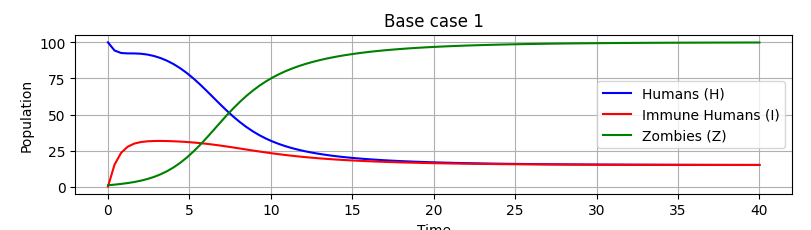
\includegraphics[width=\textwidth]{base case.png}. \\
Even when there are more zombies than humans to begin with, humans are not eradicated. As can be seen below, the zombie population stabilizes at 100 and immune and non-immune humans stabilize at 15.\\
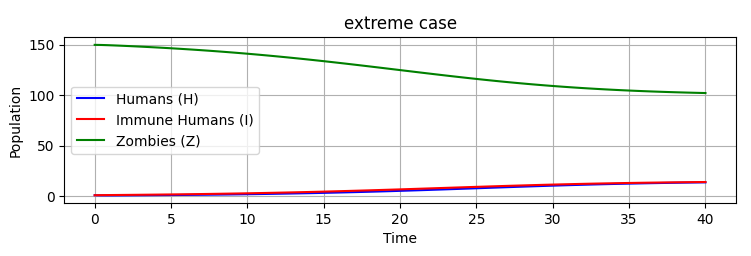
\includegraphics[width=\textwidth]{extreme case.png}.\\
\subsection{Modifications}
In order to increase chances of survival for humanity, there are several factors that can be improved. \\
First, let's assume that humans manage to distribute vaccines faster, that is, the immunization rate is increased. For instance, if instead of an immunization rate of 0.5 we increase it to 2, then the zombie population dies out, even if there are only 1 human and 100 zombies to start with:
\\
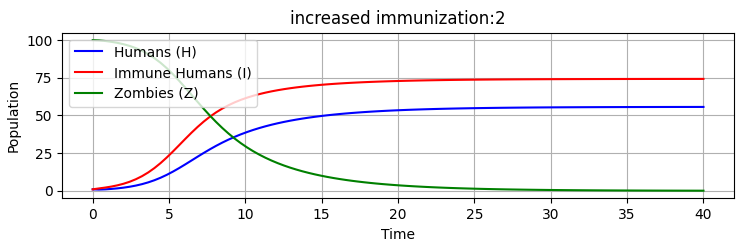
\includegraphics[width= \textwidth]{increased immunization.png}
\\
The zombification rate, however, has an even greater effect. Say, humans manage to build safer shelters, wash their hands after contact with a zombie or manage to contain zombies in specific areas, chances of survival go up. Even if zombies are infecting people with a rate of 0.01 insteadof 0.02, the human population consistently wins over the zombies.\\
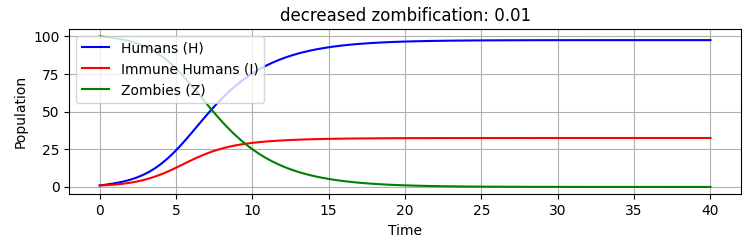
\includegraphics[width= \textwidth]{zombification.png}\\
The highest impact has an increased kill rate, however, has the most significant impact. By killing at a rate of 0.015 instead of 0.01, humanity can eradicate the zombie population:\\
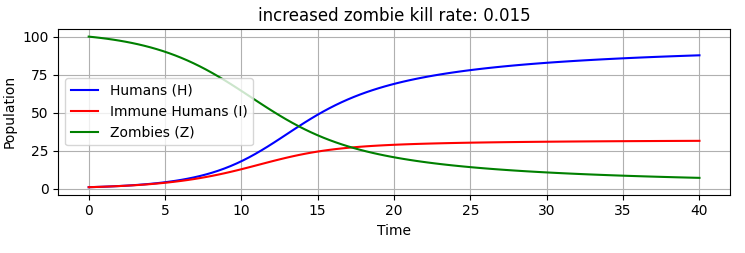
\includegraphics[width= \textwidth]{zombie kill rate.png}\\
Thus, in the case of an apocalypse, humanity should first kill more zombies, then limit the spread by building better shelters and lastly focus on increasing vaccination rates, since this rate would have to be increased by factor 4 to see a significant effect.

\section{Conclusion}

\section{Appendix}

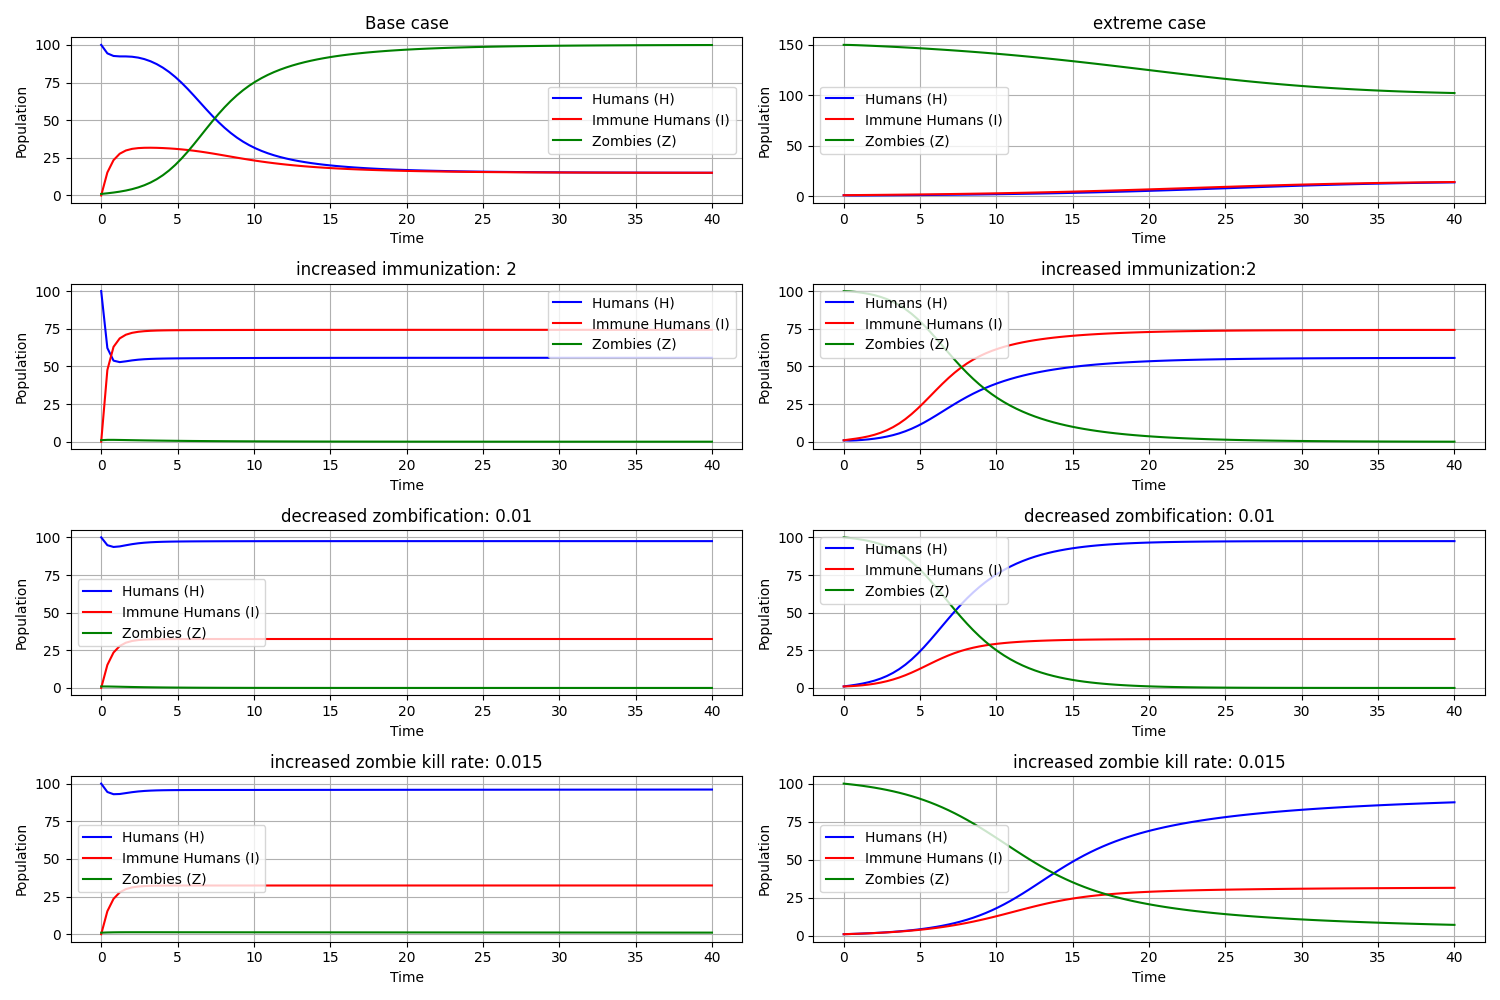
\includegraphics[width=\textwidth]{comparison of apocalypse 2.png}

\end{document}
